\documentclass{article}
\usepackage{tikz}
\usetikzlibrary{mindmap}

\begin{document}

\section{Izbira modela}
\subsection{Osrednja arhitektura}
\begin{itemize}
    \item{Pristopi so bili ovrednoteni posamično, s predpostavko medsebojne neodvisnosti (zaradi zahtevnosti treniranja)}
    \item{Modeli vrednoteni relativno med vozlišči na istem nivoju grafa}

    \item{Označbe metod:}
    \begin{itemize}
        \item{Siva - nepreizkušeno}
        \item{Zelena - izbrano za končni model}
        \item{Rdeča - neizbrano/slabše}
        \item{Modra - primerjava ni nujno primerna}
        \item{Rumena - ne predstavlja opazne izboljšave}
    \end{itemize}
\end{itemize}

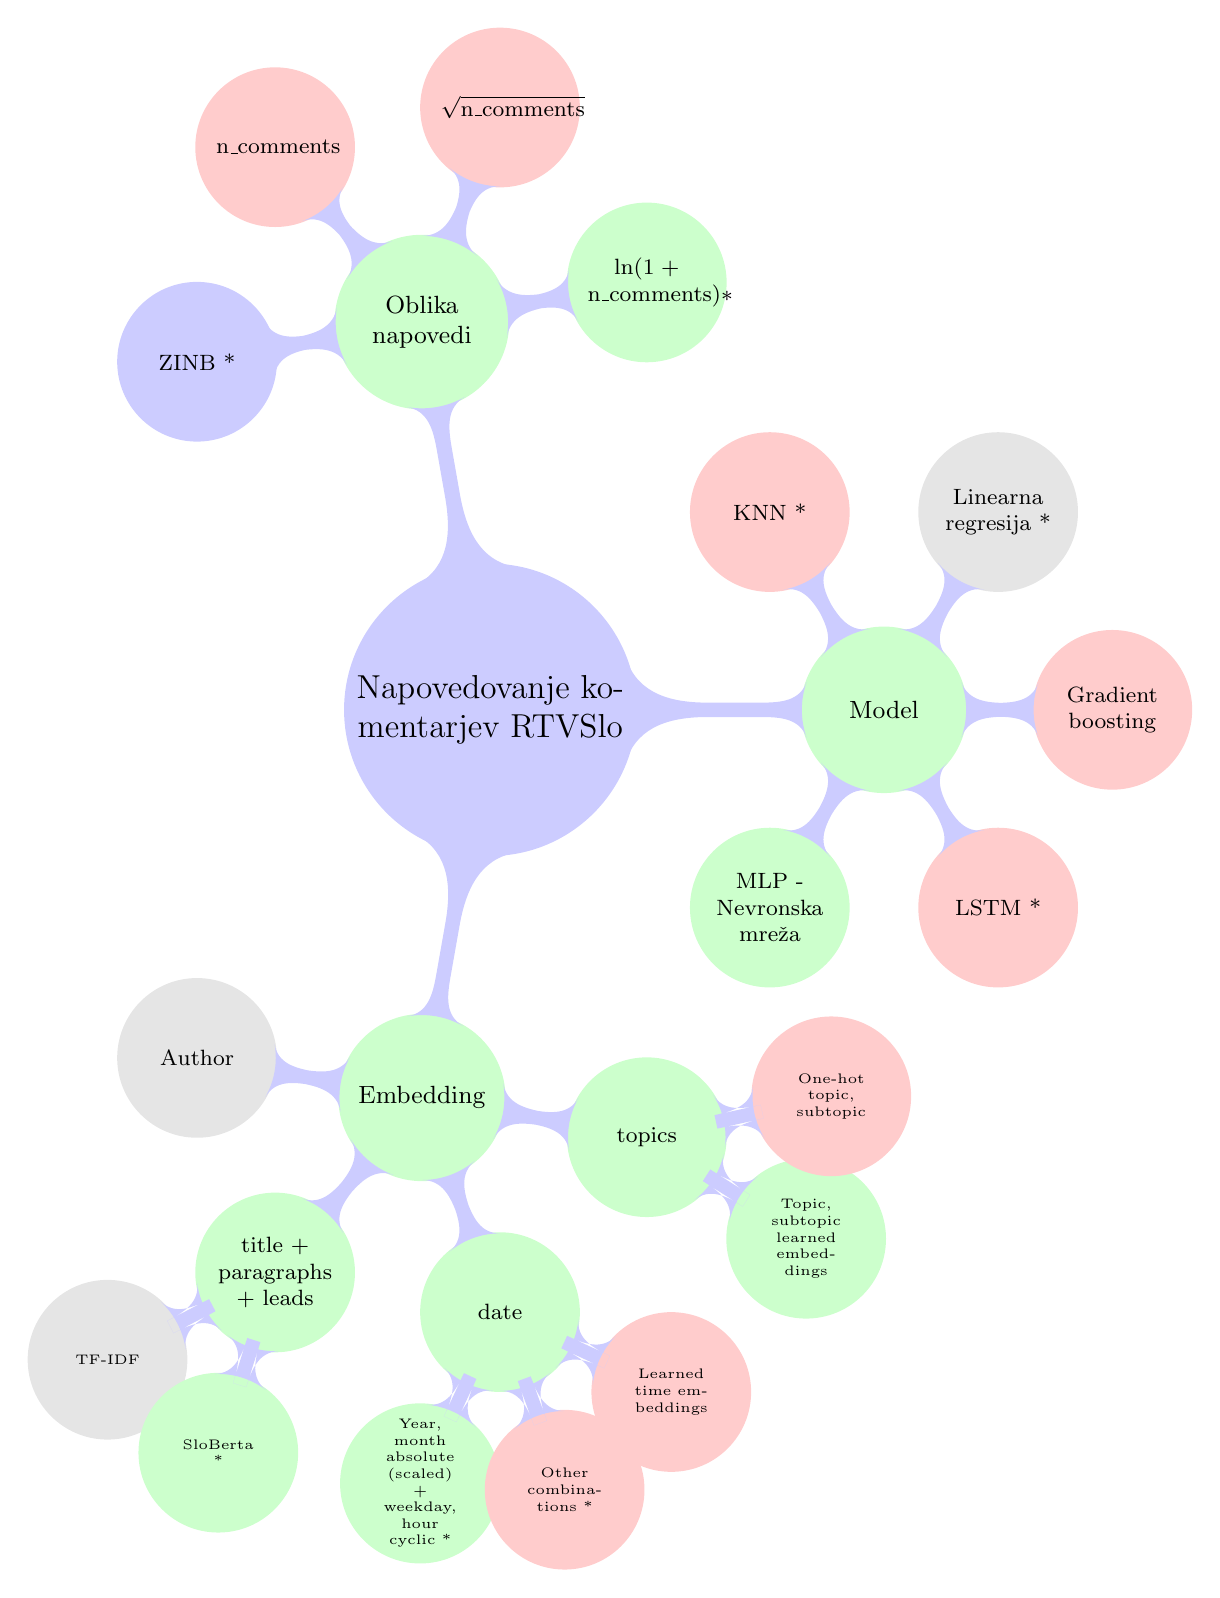
\begin{tikzpicture}[mindmap,
    every node/.style={concept, draw, circle, thick, text=black, minimum size=2cm},
    concept color=blue!20,
    grow cyclic,
    level 1/.append style={sibling angle=100},
    level 2/.append style={sibling angle=60},
    level 3/.append style={sibling angle=45},
    ]
  \node {Napovedovanje komentarjev RTVSlo}
      child { node[concept color=green!20] {Embedding}
          child { node[concept color=gray!20] {Author} }
          child { node[concept color=green!20] {title + paragraphs + leads}
              child { node[concept color=gray!20] {TF-IDF} }
              child { node[concept color=green!20] {SloBerta *} }
          }
          child { node[concept color=green!20] {date}
              child { node[concept color=green!20] {Year, month absolute (scaled) + weekday, hour cyclic *} }
              child { node[concept color=red!20] {Other combinations *} }
              child { node[concept color=red!20] {Learned time embeddings} }
          }
          child { node[concept color=green!20] {topics}
              child { node[concept color=green!20] {Topic, subtopic learned embeddings} }
              child { node[concept color=red!20] {One-hot topic, subtopic} }
          }
        }
      child { node[concept color=green!20] {Model}
          child { node[concept color=green!20] {MLP - Nevronska mreža} }
          child { node[concept color=red!20] {LSTM *} }
          child { node[concept color=red!20] {Gradient boosting} }
          child { node[concept color=gray!20] {Linearna regresija *} }
          child { node[concept color=red!20] {KNN *} }
        }
      child { node[concept color=green!20] {Oblika napovedi}
          child { node[concept color=green!20] {$\ln(1 + \mathrm{n\_comments})*$} }
          child { node[concept color=red!20] {$\sqrt{\mathrm{n\_comments}}$} }
          child { node[concept color=red!20] {n\_comments} }
          child { node[concept color=blue!20] {ZINB *} }
        };

\end{tikzpicture}

\subsection{Nadgradnje in ostale analize}
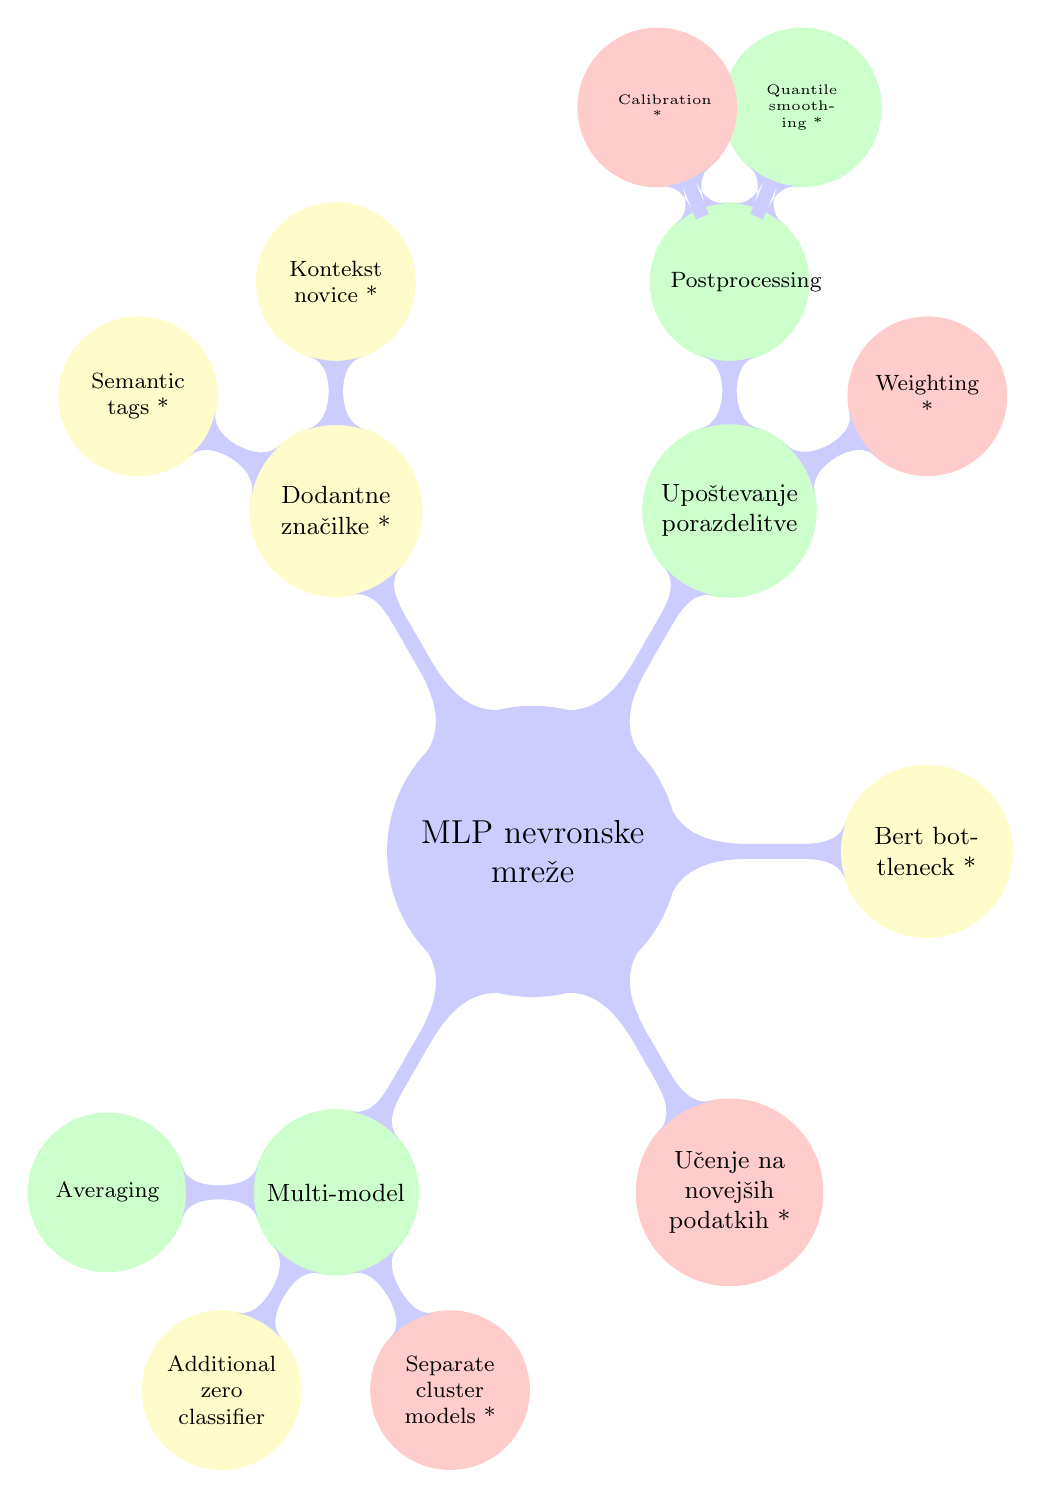
\begin{tikzpicture}[mindmap,
    every node/.style={concept, draw, circle, thick, text=black, minimum size=2cm},
    concept color=blue!20,
    grow cyclic,
    level 1/.append style={sibling angle=60},
    level 2/.append style={sibling angle=60},
    level 3/.append style={sibling angle=45},
    ]
  \node {MLP nevronske mreže}
      child { node[concept color=green!20] {Multi-model}
          child { node[concept color=green!20] {Averaging} }
          child { node[concept color=yellow!20] {Additional zero classifier} }
          child { node[concept color=red!20] {Separate cluster models *} }
        }
      child { node[concept color=red!20] {Učenje na novejših podatkih *} }
      child { node[concept color=yellow!20] {Bert bottleneck *} }
      child { node[concept color=green!20] {Upoštevanje porazdelitve} 
          child { node[concept color=red!20] {Weighting *} }
          child { node[concept color=green!20] {Postprocessing} 
              child { node[concept color=green!20] {Quantile smoothing *} }
              child { node[concept color=red!20] {Calibration *}}
          }
        }
      child { node[concept color=yellow!20] {Dodantne značilke *} 
          child { node[concept color=yellow!20] {Kontekst novice *} }
          child { node[concept color=yellow!20] {Semantic tags *} }
        };
\end{tikzpicture}

\section{Vrednotenje}
\section{Razlaga}


\end{document}

